\documentclass[12pt]{article}
\usepackage[scaled]{helvet}
\renewcommand\familydefault{\sfdefault} 
\usepackage[T1]{fontenc}

\usepackage[english]{babel}
\usepackage[utf8]{inputenc}
\usepackage{amsmath}
\usepackage{bm}
\usepackage{parskip}
\usepackage{graphicx}
\usepackage{listings}

\title{\textbf{Practical 2: Newtonian Physics}}
\author{Babis Koniaris}
\date{}

\begin{document}
\maketitle

\begin{center}
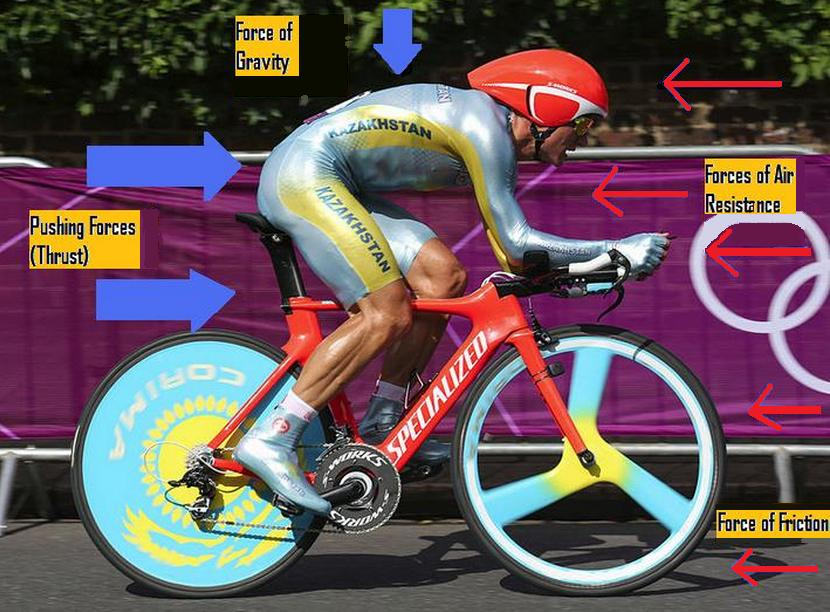
\includegraphics[width=\textwidth,height=\textheight,keepaspectratio]{p2-teaser.png}
\end{center}
\pagebreak

\section*{Introduction}

The goals of this practical are to:

\begin{itemize}
\item Give you an opportunity to become familiar with the Object-Oriented Programming framework (OOP) code that is provided to you.
\item Develop a practical understanding of particle simulations
\end{itemize}

\section*{Architecture}

The code provided to you this week has evolved using an OOP approach. Whereas last week you focussed on implement some basic particle animations, this week's main challenge is to understand and extend the given framework to run a \emph{dynamic} particle simulation. The OOP approach here allows us to use more intuitive abstractions. The project that you're going to be using is ``02\_particles\_framework''. There, you can find the several classes, split into two groups:

The first group are classes that you don't have to change their code at all for your physics simulation (nobody is stopping you however from modifying them, if you wish to):

\begin{itemize}
\item \textbf{Application}: This class contains the main application logic, is responsible for the window, input, and any other global application state (such as physics and objects)
\item \textbf{Mesh}: This class represents a 3D mesh (vertices, normals indices and associated GPU buffer information)
\item \textbf{Shader}: This class represents a GPU shader program (vertex and fragment shaders)
\item \textbf{Camera}: This class represents a camera in the virtual world
\end{itemize}

The second group are classes that you need to modify to complete the required tasks:

\begin{itemize}
\item \textbf{PhysicsEngine}: This class represents the physics state: it stores all physics objects and has code to simulate their movement.
\item \textbf{PhysicsBody}: This class represents a basic physics object. It stores a pointer to a mesh (the 3D data that make up the object), a pointer to a shader (how should we display the object), a colour (to assist with visualisation), and transformation data: position, scale and orientation. We can use this class to represent immovable objects, such as the ground plane.
\item \textbf{Particle}: This subclass is derived from a physics object, and adds a few extra variables to track necessary state, such as mass and velocity, that is needed for dynamic simulation.
\end{itemize}

This framework design is just an example one, and is by no means definitive. After the end of this module, you will possibly have your own ideas on how the framework should be changed to better support whatever physics simulation idea you have in mind! 

\subsection*{Application flow}

Our main() function is simply the creation of an Application object and running a function called MainLoop() on it. The MainLoop function first initialises the window and input, then initialises the mesh and shader databases, and finally initialises the physics engine, before entering the game loop. 

\textbf{Sidenote}: We are using mesh and shader databases to avoid duplication of objects: if every particle needs a non-modifiable reference to a mesh and a shader, we don't need to instantiate unique ones per particle, we can just reuse a single one! For example, instead of creating 100 cubes for each of 100 particles, we can reference the same cube, and use a transformation matrix to place it appropriately in the scene. The transformation matrix is the quantity that is required per-particle, not the actual mesh data, which are shared among particles. Assigning meshes and shaders to particles are the only actions that involve use of pointers in this module, and you will not be required to do any dynamic memory allocation using new/delete/malloc or smart pointers.

In the main loop we do the following:

\begin{itemize}
\item Keep track of time
\item Handle window/input events in the application
\item Handle key events in the PhysicsEngine class (\textbf{you can modify this to suit your needs!})
\item Handle input events related to camera movement
\item Generate view/projection matrices
\item Update the physics engine state
\item Draw the objects in the physics engine (this normally would be considered bad design, but is done to keep code simple, compared to introducing more classes and more complex code)
\end{itemize}

\subsection*{General coding responsibilities}

For the tasks this week and all other weeks, there are a few common things that you need to be doing:

\begin{itemize}
\item Adding variables in the physics engine class (in the class body, not global variables)
\item Initialising variables in the PhysicsEngine::Init function
\item Updating the physics state in the PhysicsEngine::Update function
\item For interactive experiments, handle keys in PhysicsEngine::HandleInputKey
\item To display any new objects, add relevant code in PhysicsEngine::Display (see example code)
\end{itemize}

Of course at various points you might need to introduce new member variables and functions in the PhysicsEngine class (or even in Particle/PhysicsBody classes) if you see fit to do so. The framework is designed to guide you, but not be overly restrictive.


\section*{Dynamic simulation}

This section is very important, as it describes the sequence of actions that makes a dynamic particle simulation. It is based on two key concepts that will be discussed in more detail in the next lecture, but that this summary should allow you to implement: Newton's second law and numerical integration

\subsection*{Newton's second law}

Most of you will be familiar with the famous equation:

\begin{align}
\bm{F} = m\bm{a}
\end{align}

This is all we need to carry out particle simulations: a link between forces applied to a particle and its acceleration. For the time being, the only force that we know applies to the particles, that we need to simulate, is gravity. In the uniform gravity field of earth, we have:

\begin{align}
\bm{F}_g = m\bm{g}
\end{align}

where:

\begin{align}
\bm{g} = (0,-9.81,0) \text{ } ms^{-2}
\end{align}

If we knew of other forces, for example aerodynamic drag ($\bm{F}_a$) or friction ($\bm{F}_f$), we would just add them up:

\begin{align}
\bm{F}=\bm{F}_g+\bm{F}_a+\bm{F}_f
\end{align}

\subsection*{Numerical integration}

Once we know the acceleration of a particle, we can obtain its velocity and position by integration. Remember, $\bm{v}$ is the derivative of $\bm{r}$ ($\bm{v} = d\bm{r}/dt$) and $\bm{a}$ is the derivative of $\bm{v}$ ($\bm{a} = d\bm{v}/dt$). So we get $\bm{v}$ from $\bm{a}$ by integration and $\bm{r}$ from $\bm{v}$ by integration. Next week, you will learn about several numerical integration techniques. Until then, here's one you can use that will work perfectly well for the type of simulations you are implementing.

Let's call $\bm{v}_{n+1}$ the new velocity to be computed at each step and $\bm{v}_{n}$ the velocity at the previous iteration. If we adopt the same notations for the acceleration and position, we can
operate our integration as follows:

\begin{align}
\bm{v}_{n+1} &= \bm{v}_n + h\bm{a}_n \\
\bm{r}_{n+1} &= \bm{r}_n + h\bm{v}_{n+1}
\end{align}

where $h$ represents the duration of a time step (\emph{deltaTime} in the code)

\subsection*{Simulation process}

Now that you know about Newton's second law and a numerical integration method, you can implement a simulation as follows:

For each frame and particle:

\begin{itemize}
\item Add all forces applied to a particle: $\bm{F}$
\item $\bm{F} = m\bm{a}$ gives you the acceleration
\item Using an integrator (such as the one above), compute the new velocity and position of the particle.
\end{itemize}

This should be sufficient for you to complete this week's tasks.

\section*{Tasks}

This week's tasks will echo last week's in that the outcome will look similar, but the algorithms will be very different. Instead of precomputed animations and closed-form functions, you will implement genuine realtime simulations. The focus of this week is to get things to work within the given framework. 

\subsection*{Task 1: Particle simulation}

You should simulate a particle, subject only to gravity. The result should look very similar to what you did last week. For testing, try giving your particle various initial velocities, and make sure that the simulation looks like what you would expect.

\subsection*{Task 2: Particle simulation, with simple collision detection}

You should add a simple collision detection step to allow particles to bounce on the ground plane. To make it more interesting than last week, this time you are asked to implement collisions with the 6 walls of a cube in which the ball bounces. To help you implement this collision detection algorithm, you can represent the cube as two vectors:
\begin{itemize}
\item \textbf{center}. The center of the cube
\item \textbf{size}. The size of the cube (width, height, depth)
\end{itemize}

In addition to making a particle bounce around in a cubic room, amend your collision response so that energy is absorbed at every bounce. The particle should eventually come to a standstill.

You can try using the provided cube model, whose mesh is centered at $(0,0,0)$ and has a size of $2$ (so it ranges from $(-1,-1,-1)$ to $(1,1,1)$).

\subsection*{Task 3: Aerodynamic drag}

As you know, in the real world (within the earth's atmosphere), a small object is subject to more than gravity. Aerodynamic drag in particular has a considerable impact on the motion of objects traveling through a fluid (like air), the higher the velocity, the stronger the effect.

You should add aerodynamic drag to the forces applied to simulated particles.

\subsection*{Further tasks}

Here are further tasks you can complete to further your understanding of the topic:

\begin{itemize}
\item Add wind to your simulation. You can start with a simple isotropic wind that has constant velocity and take things further by varying the wind speed and then making it anisotropic i.e., not the same across the 3D space.
\item Add friction to your simulation and/or something that will ensure that your particles don't keep travelling forever. In other words, make them stop in a physically believable fashion.
\end{itemize}

%\section*{Deliverables}

%There is no deliverable for this assignment but the work you are completing this week will contribute to next week's assignment, which will be assessed. So make sure you don't lose your work.

\end{document}